\ifx\type\undefined
  \documentclass[10pt, t]{beamer}
  \setbeamertemplate{footline}[page number]
\else
  \documentclass[10pt]{article}
  \usepackage[margin=1in]{geometry}
\fi

\usepackage{amsmath}
\usepackage{amssymb}
\usepackage{amsthm}
\usepackage{bbm}
\usepackage{cancel}
\usepackage{listings}
\usepackage{mathrsfs}
\usepackage{multirow}
\usepackage{soul}
\usepackage{stmaryrd}
\usepackage{tikz}
\usepackage{tikz-cd}
\usepackage{wrapfig}

\newtheorem*{algorithm}{Algorithm}
\newtheorem*{assumptions}{Assumptions}
\newtheorem*{conjecture}{Conjecture}
\newtheorem*{consequences}{Consequences}
\newtheorem*{exercise}{Exercise}
\newtheorem*{formalisation}{Formalisation}
\newtheorem*{proposition}{Proposition}
\newtheorem*{question}{Question}
\newtheorem*{remark}{Remark}

\ifx\type\undefined\else
  \newtheorem*{definition}{Definition}
  \newtheorem*{example}{Example}
  \newtheorem*{lemma}{Lemma}
  \newtheorem*{theorem}{Theorem}
\fi

\definecolor{keywordcolor}{rgb}{0.7, 0.1, 0.1}
\definecolor{tacticcolor}{rgb}{0.0, 0.1, 0.6}
\definecolor{commentcolor}{rgb}{0.4, 0.4, 0.4}
\definecolor{symbolcolor}{rgb}{0.0, 0.1, 0.6}
\definecolor{sortcolor}{rgb}{0.1, 0.5, 0.1}
\definecolor{attributecolor}{rgb}{0.7, 0.1, 0.1}
\def\lstlanguagefiles{lstlean.tex}
\lstset{language=lean}

\newcommand\A{\mathbb{A}}
\newcommand\C{\mathbb{C}}
\newcommand\F{\mathbb{F}}
\newcommand\G{\mathbb{G}}
\renewcommand\H{\mathbb{H}}
\newcommand\I{\mathbb{I}}
\newcommand\N{\mathbb{N}}
\renewcommand\P{\mathbb{P}}
\newcommand\Q{\mathbb{Q}}
\newcommand\R{\mathbb{R}}
\newcommand\Z{\mathbb{Z}}

\renewcommand\AA{\mathcal{A}}
\newcommand\BB{\mathcal{B}}
\newcommand\CC{\mathcal{C}}
\newcommand\DD{\mathcal{D}}
\newcommand\EE{\mathcal{E}}
\newcommand\FF{\mathcal{F}}
\newcommand\GG{\mathcal{G}}
\newcommand\HH{\mathcal{H}}
\newcommand\II{\mathcal{I}}
\newcommand\LL{\mathcal{L}}
\newcommand\MM{\mathcal{M}}
\newcommand\NN{\mathcal{N}}
\newcommand\OO{\mathcal{O}}
\newcommand\PP{\mathcal{P}}
\newcommand\RR{\mathcal{R}}
\renewcommand\SS{\mathcal{S}}
\newcommand\TT{\mathcal{T}}
\newcommand\XX{\mathcal{X}}

\renewcommand\aa{\mathfrak{a}}
\newcommand\cc{\mathfrak{c}}
\newcommand\dd{\mathfrak{d}}
\newcommand\ff{\mathfrak{f}}
\renewcommand\gg{\mathfrak{g}}
\newcommand\mm{\mathfrak{m}}
\newcommand\pp{\mathfrak{p}}
\newcommand\qq{\mathfrak{q}}
\renewcommand\ss{\mathfrak{s}}

\newcommand\LLL{\mathscr{L}}

\newcommand\ab{\mathrm{ab}}
\newcommand\Ab{\mathbf{Ab}}
\newcommand\Alg{\mathbf{Alg}}
\newcommand\Aff{\mathbf{Aff}}
\newcommand\Aut{\operatorname{Aut}}
\newcommand\Az{\mathrm{Az}}
\newcommand\Br{\operatorname{Br}}
\newcommand\BSD{\operatorname{BSD}}
\newcommand\ch{\operatorname{char}}
\newcommand\Cl{\operatorname{Cl}}
\newcommand\coker{\operatorname{coker}}
\newcommand\cris{\mathrm{cris}}
\renewcommand\d{\mathrm{d}}
\newcommand\Div{\operatorname{Div}}
\newcommand\dR{\mathrm{dR}}
\newcommand\EN{\operatorname{EN}}
\newcommand\End{\operatorname{End}}
\newcommand\ES{\operatorname{ES}}
\newcommand\et{\mathrm{\acute{e}t}}
\newcommand\Et{\mathbf{\acute{E}t}}
\newcommand\Ext{\operatorname{Ext}}
\newcommand\Fr{\operatorname{Fr}}
\newcommand\Frac{\operatorname{Frac}}
\newcommand\Gal{\operatorname{Gal}}
\newcommand\GL{\operatorname{GL}}
\newcommand\Gr{\mathrm{Gr}}
\newcommand\Hom{\operatorname{Hom}}
\newcommand\HT{\mathrm{HT}}
\newcommand\id{\operatorname{id}}
\newcommand\im{\operatorname{im}}
\newcommand\Ind{\operatorname{Ind}}
\renewcommand\inf{\operatorname{inf}}
\newcommand\inv{\operatorname{inv}}
\newcommand\Irr{\operatorname{Irr}}
\newcommand\Jac{\operatorname{Jac}}
\newcommand\lcm{\operatorname{lcm}}
\newcommand\Mat{\operatorname{Mat}}
\newcommand\Mod{\mathbf{Mod}}
\newcommand\Nm{\operatorname{Nm}}
\newcommand\nr{\mathrm{nr}}
\newcommand\NS{\operatorname{NS}}
\newcommand\Ob{\operatorname{Ob}}
\newcommand\ord{\operatorname{ord}}
\newcommand\op{\mathrm{op}}
\newcommand\PGL{\operatorname{PGL}}
\newcommand\Pic{\operatorname{Pic}}
\newcommand\Prob{\operatorname{Prob}}
\newcommand\Proj{\operatorname{Proj}}
\newcommand\PSh{\mathbf{PSh}}
\newcommand\Reg{\operatorname{Reg}}
\newcommand\res{\operatorname{res}}
\newcommand\rk{\operatorname{rk}}
\newcommand\Sch{\mathbf{Sch}}
\newcommand\Sel{\operatorname{Sel}}
\newcommand\Set{\mathbf{Set}}
\newcommand\sgn{\operatorname{sgn}}
\newcommand\Sh{\mathbf{Sh}}
\newcommand\SL{\operatorname{SL}}
\newcommand\Spec{\operatorname{Spec}}
\newcommand\supp{\operatorname{supp}}
\newcommand\Tam{\operatorname{Tam}}
\newcommand\Top{\mathbf{Top}}
\newcommand\tor{\operatorname{tor}}
\newcommand\tr{\operatorname{tr}}
\newcommand\tra{\operatorname{tra}}
\newcommand\WC{\operatorname{WC}}

\DeclareFontFamily{U}{wncyr}{}
\DeclareFontShape{U}{wncyr}{m}{n}{<->wncyr10}{}
\DeclareSymbolFont{cyr}{U}{wncyr}{m}{n}
\DeclareMathSymbol{\Sha}{\mathord}{cyr}{"58}

\newcommand{\function}[5][]{
  \if &#1&
    \begin{array}{rcl}
      #2 & \longrightarrow & #3 \\
      #4 & \longmapsto     & #5
    \end{array}
  \else
    \begin{array}{rcrcl}
      #1 & : & #2 & \longrightarrow & #3 \\
         &   & #4 & \longmapsto     & #5
    \end{array}
  \fi
}

\newcommand{\functions}[7][]{
  \if &#1&
    \begin{array}{rcl}
      #2 & \longrightarrow & #3 \\
      #4 & \longmapsto     & #5 \\
      #6 & \longmapsto     & #7 \\
    \end{array}
  \else
    \begin{array}{rcrcl}
      #1 & : & #2 & \longrightarrow & #3 \\
         &   & #4 & \longmapsto     & #5 \\
         &   & #6 & \longmapsto     & #7
    \end{array}
  \fi
}
\title{Computing Euler factors}
\subtitle{Models of curves and arithmetic applications}
\author{David Kurniadi Angdinata}
\institute{University College London}
\date{Wednesday, 2 April 2025}

\begin{document}

\frame\maketitle

\begin{frame}[c]{Notation}

\begin{itemize}
\item[$ p $] an odd prime (of almost good reduction)
\item[$ C $] a smooth projective (hyperelliptic) curve of genus $ g $ ($ = 2 $) over $ \Q $ (with semistable reduction at $ p $) given by an integral model
$$ Y^2 = c\prod_{r \in \RR} (X - r), \qquad c \in \Z, \qquad r \in \overline{\Q}. $$
\item[$ \CC $] the minimal regular model of $ C $ at $ p $
\item[$ \widetilde{\CC} $] the special fibre of $ \CC $
\item[$ \overline{C} $] the base change of $ C $ to $ \overline{\Q} $
\item[$ \overline{\widetilde{\CC}} $] the base change of $ \widetilde{\CC} $ to $ \overline{\F_p} $
\end{itemize}

\end{frame}

\begin{frame}{L-functions}

Recall that the L-function of $ C $ is the Euler product
$$ L(C, s) := \prod_p \dfrac{1}{L_p(C, p^{-s})}, $$
over all primes $ p $, where the local Euler factor at $ p $ is the polynomial
$$ L_p(C, T) := \det(1 - T \cdot \Fr_p^{-1} \mid H_\et^1(\overline{C}, \Q_\ell)^{I_p}). $$
When $ C $ has semistable reduction at $ p $,
$$ H_\et^1(\overline{C}, \Q_\ell)^{I_p} \cong H_\et^1(\overline{\widetilde{\CC}}, \Q_\ell), $$
which is an isomorphism of $ \Gal(\overline{\Q_p} / \Q_p) $-representations, so that
$$ L_p(C, T) = \det(1 - T \cdot \Fr_p^{-1} \mid H_\et^1(\overline{\widetilde{\CC}}, \Q_\ell)). $$
This can be extracted from the $ \zeta $-function of $ \widetilde{\CC} $.

\end{frame}

\begin{frame}{$ \zeta $-functions}

The $ \zeta $-function of a projective curve $ X $ over $ \F_p $ is the rational function
$$ \zeta(X, T) := \exp\left(\sum_{k \ge 1} \#X(\F_{p^k})\dfrac{T^k}{k}\right) = \dfrac{P_1(X, T)}{P_0(X, T) \cdot P_2(X, T)}, $$
by the Weil conjectures, where
$$ P_i(X, T) := \det(1 - T \cdot \Fr_p^{-1} \mid H_\et^1(X, \Q_\ell)), \qquad i = 0, 1, 2. $$
When the Jacobian $ \Jac(C) $ of $ C $ has good reduction at $ p $,
$$ P_0(\widetilde{\CC}, T) = 1 - T, \qquad \deg P_1(\widetilde{\CC}, T) = 2g, \qquad P_2(\widetilde{\CC}, T) = 1 - pT, $$
so that $ L_p(C, T) $ is determined by $ \#\widetilde{\CC}(\F_{p^k}) $ for sufficiently many $ k \ge 1 $.

\bigskip In general, this requires computing the minimal regular model $ \CC $ by a resolution of singularities, which is computationally expensive.

\end{frame}

\begin{frame}{Cluster pictures}

Instead of computing $ \CC $, its special fibre $ \widetilde{\CC} $ can be recovered from cluster picture machinery, with explicit models for its irreducible components.

\bigskip Recall that a cluster is a non-empty subset of $ \RR $ of the form
$$ \ss = \{r \in \RR : \nu_p(r - z) \ge d\}, \qquad z \in \overline{\Q_p}, \qquad d \in \Q. $$
The depth $ d_\ss $ of a cluster $ \ss $ is the largest such $ d $, in which case any $ z $ with $ \nu_p(r - z) = d_\ss $ for some $ r \in \ss $ is called a centre $ z_\ss $ of $ \ss $. A child of $ \ss $ is a maximal subcluster $ \ss' \subsetneq \ss $, and its relative depth $ \delta_{\ss'} $ is simply $ d_{\ss'} - d_\ss $.

\bigskip A cluster $ \ss $ is called odd or even if $ |\ss| $ is odd or even respectively. It is called \"ubereven if every child of $ \ss $ is even. It is called twin if $ |\ss| = 2 $, and it is called cotwin if it is not \"ubereven but it has a child $ \ss' $ with $ |\ss'| = 2g $.

\bigskip The cluster $ \RR $ is called principal if it is odd or if it has more than two children. In general, a cluster $ \ss $ is called principal when $ |\ss| \ge 3 $ but has no children $ \ss' $ with $ |\ss'| = 2g $.

\end{frame}

\begin{frame}{Cluster picture example}

Let $ C $ be the hyperelliptic curve over $ \Q $ given by
$$ Y^2 = 2X(X - 1)(X - p^n)(X - 2p^n)(X - p^m)(X - 2p^m), $$
where $ p $ is an odd prime and $ m \ge n $ are positive integers.

\bigskip The associated cluster picture is:
$$
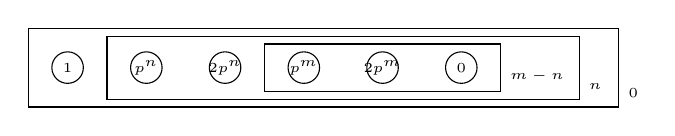
\begin{tikzpicture}
\draw (0, 0) rectangle (7.5, -1) node[above right]{\tiny $ 0 $};
\draw (0.5, -0.5) circle (0.2) node{\tiny $ 1 $};
\draw (1, -0.1) rectangle (7, -0.9) node[above right]{\tiny $ n $};
\draw (1.5, -0.5) circle (0.2) node{\tiny $ p^n $};
\draw (2.5, -0.5) circle (0.2) node{\tiny $ 2p^n $};
\draw (3, -0.2) rectangle (6, -0.8) node[above right]{\tiny $ m - n $};
\draw (3.5, -0.5) circle (0.2) node{\tiny $ p^m $};
\draw (4.5, -0.5) circle (0.2) node{\tiny $ 2p^m $};
\draw (5.5, -0.5) circle (0.2) node{\tiny $ 0 $};
\end{tikzpicture}
$$
The cluster $ \RR $ is not principal, but it has two principal subclusters.
\begin{itemize}
\item The odd subcluster $ \ss_m := \{p^m, 2p^m, 0\} $ has centre $ z_{\ss_m} = 0 $, depth $ d_{\ss_m} = m $ and relative depth $ \delta_{\ss_m} = m - n $.
\item The odd subcluster $ \ss_n := \{p^n, 2p^n, p^m, 2p^m, 0\} $ has centre $ z_{\ss_n} = p^n $, depth $ d_{\ss_n} = n $, and relative depth $ \delta_{\ss_n} = n $.
\end{itemize}
Neither subclusters are \"ubereven or cotwin.

\end{frame}

\begin{frame}{Components of special fibres}

\begin{theorem}[M2D2, Theorem 8.6(1)]
Let $ C $ be a hyperelliptic curve over $ \Q $ given by
$$ Y^2 = c\prod_{r \in \RR} (X - r), \qquad c \in \Z, \qquad r \in \overline{\Q}. $$
Assume that $ C $ has semistable reduction at some odd prime $ p $, and that $ \delta_\ss \ne \tfrac{1}{2} $ for any principal cluster $ \ss $. Then the components of $ \widetilde{\CC} $ consist of the curves $ \Gamma_\ss $ associated to principal clusters $ \ss $, given by
$$ Y^2 = \widetilde{\dfrac{c}{p^{\nu_p(c)}}}\prod_{r \in \RR \setminus \ss} \widetilde{\dfrac{z_\ss - r}{p^{\nu_p(z_\ss - r)}}}\prod_{\text{odd} \ \ss' < \ss} \left(X - \widetilde{\dfrac{z_{\ss'} - z_\ss}{p^{d_\ss}}}\right). $$
This is irreducible except when $ \ss $ is \"ubereven, in which case it has two irreducible components $ \Gamma_\ss^+ $ and $ \Gamma_\ss^- $. The remaining components of $ \widetilde{\CC} $ are chains of $ \P^1 $ that link $ \Gamma_\ss $, which are given by the following conditions.
\end{theorem}

\end{frame}

\begin{frame}{Intersections of special fibres}

\begin{theorem}[M2D2, Theorem 8.6(1), continued]
\begin{itemize}
\item Assume that $ \ss' < \ss $.
\begin{itemize}
\item When $ \ss' $ is principal odd and $ \ss $ is principal, then there is a chain from $ \Gamma_{\ss'} $ to $ \Gamma_\ss $ of length $ \tfrac{1}{2}\delta_{\ss'} - 1 $.
\item When $ \ss' $ is principal even and $ \ss $ is principal, then there are two chains from $ \Gamma_{\ss'}^+ $ to $ \Gamma_\ss^+ $ and from $ \Gamma_{\ss'}^- $ to $ \Gamma_\ss^- $ each of length $ \delta_{\ss'} - 1 $.
\item When $ \ss' $ is twin and $ \ss $ is principal, then there is a chain from $ \Gamma_\ss^- $ to $ \Gamma_\ss^+ $ of length $ 2\delta_{\ss'} - 1 $.
\item When $ \ss' $ is principal and $ \ss $ is cotwin, then there is a chain from $ \Gamma_{\ss'}^- $ to $ \Gamma_{\ss'}^+ $ of length $ 2\delta_{\ss'} - 1 $.
\end{itemize}
\item Assume that $ \RR $ is not principal, but $ \RR = \ss_1 \sqcup \ss_2 $.
\begin{itemize}
\item When $ \ss_1 $ and $ \ss_2 $ are principal odd, then there is a chain from $ \Gamma_{\ss_1} $ to $ \Gamma_{\ss_2} $ of length $ \tfrac{1}{2}(\delta_{\ss_1} + \delta_{\ss_2}) - 1 $.
\item When $ \ss_1 $ and $ \ss_2 $ are principal even, then there are two chains from $ \Gamma_{\ss_1}^+ $ to $ \Gamma_{\ss_2}^+ $ and from $ \Gamma_{\ss_1}^- $ to $ \Gamma_{\ss_2}^- $ each of length $ \delta_{\ss_1} + \delta_{\ss_2} - 1 $.
\item When $ \ss_1 $ is principal even and $ \ss_2 $ is twin, then there is a chain from $ \Gamma_{\ss_1}^- $ to $ \Gamma_{\ss_1}^+ $ of length $ 2(\delta_{\ss_1} + \delta_{\ss_2}) - 1 $.
\end{itemize}
\end{itemize}
\end{theorem}

\end{frame}

\begin{frame}{Special fibre example}

Continuing on the previous example, $ \Gamma_{\ss_m} $ computes to be
\begin{align*}
Y^2 & = 2\widetilde{\left(\dfrac{0 - 1}{p^{\nu_p(0 - 1)}}\right)}\widetilde{\left(\dfrac{0 - p^n}{p^{\nu_p(0 - p^n)}}\right)}\widetilde{\left(\dfrac{0 - 2p^n}{p^{\nu_p(0 - 2p^n)}}\right)} \\
& \qquad \left(X - \widetilde{\dfrac{p^m - 0}{p^m}}\right)\left(X - \widetilde{\dfrac{2p^m - 0}{p^m}}\right)\left(X - \widetilde{\dfrac{0 - 0}{p^m}}\right) \\
& = -4X(X - 1)(X - 2),
\end{align*}
and $ \Gamma_{\ss_n} $ computes to be
\begin{align*}
Y^2 & = 2\widetilde{\left(\dfrac{p^n - 1}{p^{\nu_p(p^n - 1)}}\right)}\left(X - \widetilde{\dfrac{p^n - p^n}{p^n}}\right)\left(X - \widetilde{\dfrac{2p^n - p^n}{p^n}}\right)\left(X - \widetilde{\dfrac{0 - p^n}{p^n}}\right) \\
& = -2X(X - 1)(X + 1).
\end{align*}
Furthermore, there is a chain from $ \Gamma_{\ss_m} $ to $ \Gamma_{\ss_n} $ of length $ \tfrac{1}{2}(m - n) - 1 $.

\end{frame}

\begin{frame}{$ \zeta $-function example}

Recall that to compute $ \zeta(\widetilde{\CC}, T) $, it suffices to compute
$$ \#C(\F_{p^k}) = \#\Gamma_{\ss_m}(\F_{p^k}) + \#\Gamma_{\ss_n}(\F_{p^k}) + \left(\dfrac{m - n}{2} - 1\right)\#\P^1(\F_{p^k}) - \dfrac{m - n}{2}, $$
for all $ k \ge 1 $. For instance, if $ p = 5 $, then
\begin{align*}
\#\Gamma_{\ss_m}(\F_{5^k}) & = 1 - ((-1 - 2i)^k + (-1 + 2i)^k) + 5^k, \\
\#\Gamma_{\ss_n}(\F_{5^k}) & = 1 - ((1 - 2i)^k + (1 + 2i)^k) + 5^k,
\end{align*}
and if $ m = 16 $ and $ n = 10 $, then
$$ \#C(\F_{5^k}) = 1 + 4 \cdot 5^k - \sum_\pm (\pm1 \pm 2i)^k, $$
so that
$$ \zeta(\widetilde{\CC}, T) = \dfrac{\prod_\pm (1 - (\pm1 \pm 2i)T)}{(1 - T)(1 - 5T)^4} = \dfrac{(1 - 2T + 5T^2)(1 + 2T + 5T^2)}{(1 - T)(1 - 5T)^4}. $$

\end{frame}

\begin{frame}{Almost good primes}

Unlike elliptic curves, there are higher genus curves $ C $ over $ \Q $ with primes $ p $ that divide its minimal discriminant $ \Delta_C $ but do not divide its conductor $ \ff_C $, such as when $ \Jac(C) $ reduces to a product of elliptic curves over $ \F_p $. These primes $ p $ are called primes of \textbf{almost good reduction} for $ C $.

\bigskip For instance, the genus two curve over $ \Q $ given by
\begin{align*}
& Y^2 + (X^3 + X^2 + X)Y = -144061786290072X^6 - 23062462482396X^5 \\
& \qquad - 1266273619292236X^4 - 3052943051575761X^3 \\
& \qquad + 3989955132045666X^2 + 3438312415pX - 1707513566p
\end{align*}
has $ \ff_C = 270761 $ but $ \Delta_C = 270761p^{22} $ where $ p = 14556001 $.

\bigskip Maistret and Sutherland were motivated to expand the LMFDB, which currently contains $ 66158 $ genus two curves $ C $ over $ \Q $ with $ \Delta_C \le 10^6 $, to over $ 5 \cdot 10^6 $ genus two curves $ C $ over $ \Q $ with $ \ff_C \le 2^{20} \approx 10^6 $.

\end{frame}

\begin{frame}{Cluster pictures at almost good primes}

The prime of almost good reduction forces the existence of a subcluster of size $ 3 $, all subclusters to be odd, and specific conditions on their depths.

\begin{theorem}[MS25, Corollaries 3.5/7/10/11]
Let $ C $ be a hyperelliptic curve over $ \Q $ given by $ Y^2 = \sum_{i = 0}^6 c_iX^i \in \Z[X] $ such that $ d_\RR = 0 $ and $ \nu_p(c_6) = \min_i\nu_p(c_i) \le 1 $ at some odd prime $ p $ of almost good reduction. Then its cluster picture is one of the following:
\begin{align*}
&
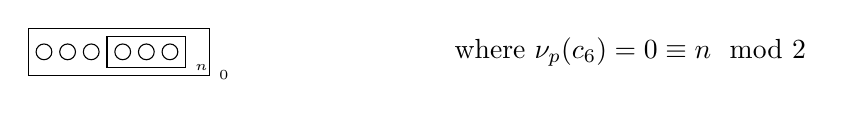
\begin{tikzpicture}
\draw (0, 0) rectangle (2.3, -0.6) node[right]{\tiny $ 0 $};
\draw (0.2, -0.3) circle (0.1);
\draw (0.5, -0.3) circle (0.1);
\draw (0.8, -0.3) circle (0.1);
\draw (1, -0.1) rectangle (2, -0.5) node[right]{\tiny $ n $};
\draw (1.2, -0.3) circle (0.1);
\draw (1.5, -0.3) circle (0.1);
\draw (1.8, -0.3) circle (0.1);
\draw (10, -0.3) node[left]{where $ \nu_p(c_6) = 0 \equiv n \mod 2 $};
\end{tikzpicture}
\\ &
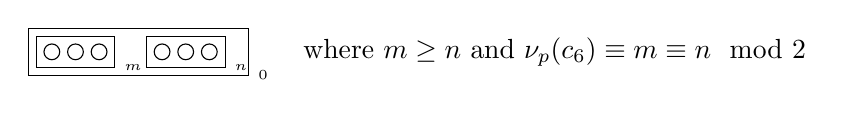
\begin{tikzpicture}
\draw (0, 0) rectangle (2.8, -0.6) node[right]{\tiny $ 0 $};
\draw (0.1, -0.1) rectangle (1.1, -0.5) node[right]{\tiny $ m $};
\draw (0.3, -0.3) circle (0.1);
\draw (0.6, -0.3) circle (0.1);
\draw (0.9, -0.3) circle (0.1);
\draw (1.5, -0.1) rectangle (2.5, -0.5) node[right]{\tiny $ n $};
\draw (1.7, -0.3) circle (0.1);
\draw (2, -0.3) circle (0.1);
\draw (2.3, -0.3) circle (0.1);
\draw (10, -0.3) node[left]{where $ m \ge n $ and $ \nu_p(c_6) \equiv m \equiv n \mod 2 $};
\end{tikzpicture}
\\ &
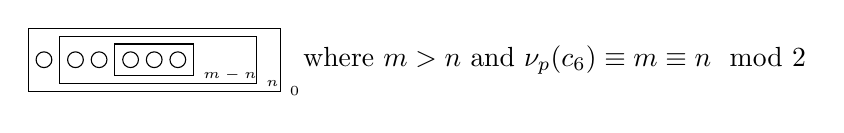
\begin{tikzpicture}
\draw (0, 0) rectangle (3.2, -0.8) node[right]{\tiny $ 0 $};
\draw (0.2, -0.4) circle (0.1);
\draw (0.4, -0.1) rectangle (2.9, -0.7) node[right]{\tiny $ n $};
\draw (0.6, -0.4) circle (0.1);
\draw (0.9, -0.4) circle (0.1);
\draw (1.1, -0.2) rectangle (2.1, -0.6) node[right]{\tiny $ m - n $};
\draw (1.3, -0.4) circle (0.1);
\draw (1.6, -0.4) circle (0.1);
\draw (1.9, -0.4) circle (0.1);
\draw (10, -0.4) node[left]{where $ m > n $ and $ \nu_p(c_6) \equiv m \equiv n \mod 2 $};
\end{tikzpicture}
\end{align*}
Furthermore, there is an explicit description for $ \widetilde{\CC} $ as the union of two elliptic curves over $ \F_{p^2} $ linked by a chain of $ \P^1 $ for each cluster picture.
\end{theorem}

\end{frame}

\begin{frame}{Computing Euler factors}

It turns out that any genus two curve over $ \Q $ with almost good reduction at an odd prime can be normalised to obtain such a model.

\begin{theorem}[MS25, Theorem 1.1]
Let $ C $ be a genus two curve over $ \Q $ given by $ Y^2 = \sum_{i = 0}^6 c_iX^i \in \Z[X] $ with almost good reduction at some odd prime $ p $. Then there is a probabilistic algorithm that computes $ L_p(C, T) $ with running time
$$ O\left(\dfrac{(\max_i\log|c_i|)^2\log^2(\max_i\log|c_i|)}{\log p} + \log^5p\right). $$
Furthermore, if a quadratic non-residue modulo $ p $ is given, then the algorithm is deterministic with the same running time.
\end{theorem}

\bigskip This has been implemented in Magma in the public \texttt{Genus2Euler} repository. In a test on $ 3454506 $ pairs of $ (C, p) $, it is almost $ 5000 $ times faster than the existing \texttt{EulerFactor} function in Magma, including $ 489 $ pairs of $ (C, p) $ whose computations were terminated after eight hours.

\end{frame}

\begin{frame}[c]{References}

\begin{itemize}
\item[MS25] C\'eline Maistret, Andrew Sutherland. Computing Euler factors of genus 2 curves at odd primes of almost good reduction. Research in Number Theory 11, 37 (2025). https://doi.org/10.1007/s40993-024-00605-7
\item[M2D2] Tim Dokchitser, Vladimir Dokchitser, C\'eline Maistret, Adam Morgan. Arithmetic of hyperelliptic curves over local fields. Mathematische Annalen 385, 1213-1322 (2023). https://doi.org/10.1007/s00208-021-02319-y
\end{itemize}

\end{frame}

\end{document}